\documentclass{article}
\usepackage[utf8]{inputenc}

\usepackage{graphicx}
\usepackage{color}

\usepackage{geometry}
\geometry{hmargin=2.5cm,vmargin=1.5cm}

\begin{document}

\begin{figure}[t]
\centering

\includegraphics[width=5cm]{inp_n7.png}
\end{figure}

\title{\vspace{4cm} \textbf{Titre du rapport}}
\author{Nom des auteurs\\ }
\date{\vspace{7cm} Département Sciences du Numérique - Première année \\
2019-2020 }

\maketitle

\newpage
\tableofcontents
\listoffigures

\newpage
%%%%%%%%%%%%%%%%%%%%%%%%%%%%%%%%%%%%%%%%%%%%%%%%%%%%%%%%%%%%%%%%%%
\section{Introduction}
%%%%%%%%%%%%%%%%%%%%%%%%%%%%%%%%%%%%%%%%%%%%%%%%%%%%%%%%%%%%%%%%%%
\subsection{Objectifs du travail réalisé}
\textcolor{blue}{A compléter}

\subsection{Schéma général des chaines à étudier (canal AWGN)}
La figure \ref{chaine_ex1} présente le schéma général des chaines à étudier.

\begin{figure}[ht!]
\centering
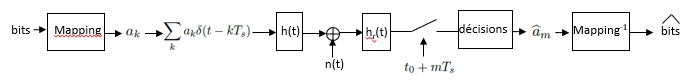
\includegraphics[width=15cm]{figure1.png}
\caption{Chaîne de transmission en bande de base}.
\label{chaine_ex1}
\end{figure}

\subsubsection{Génération de l'information binaire à transmettre}
La génération de l'information binaire à transmettre (bits $0$ et $1$ équiprobables et indépendants) pourra être réalisée grâce à la fonction \emph{randi} de Matlab.
%Mais ses éléments peuvent aussi provenir d'un texte ou d'une image.\\
%Pour associer une information binaire à un texte (et un texte à une information binaire), vous pouvez, par exemple, utiliser les lignes de code matlab suivantes :
%\begin{itemize}
%\item Bits=double(str2bin('Texte')).';
%\item ...
%\item TexteRecu=bin2str(BitsRecus);
%\end{itemize}
%
%Pour associer une information binaire à une image noir et blanc (et une image noir et blanc à une information binaire), vous pouvez, par exemple, utiliser les lignes de code matlab suivantes :
%\begin{itemize}
%\item Image = imread('barbara.png');
%\item ImageBinaire=de$2$bi(Image);
%\item VecteurBinaire=double(reshape(ImageBinaire.',$1$,size(ImageBinaire,$1$)*size(ImageBinaire,$2$)));
%\item ...
%\item xx=reshape(BitsRecus,size(ImageBinaire,$2$),size(ImageBinaire,$1$));
%\item ImageRecue=reshape(bi$2$de(xx.'),size(Image,1),length(xx)/size(Image,$1$));
%\item figure; imagesc(ImageRecue); colormap('gray');
%\end{itemize}

%Remarque : afin de les rendre indépendants, lorsqu'ils proviennent d'un texte ou d'une image, il peut être nécessaire d'embrouiller les bits représentant l'information à transmettre.

\subsubsection{Mapping}
Un mapping devra être réalisé afin de passer de l'information binaire aux symboles $a_k$. Le mapping est un des élements qui pourra différer selon les chaines de transmission à étudier et implanter.

\subsubsection{Suréchantillonnage}
La suite d'impulsions de Dirac espacées de la durée symbole $T_s$ et pondérées par les symboles $a_k$ issus du mapping sera générée, en numérique, en insérant $N_s-1$ zéros entre deux symboles $a_k$, si $N_s$ représente le nombre d'échantillons utilisés par symbole (ou facteur de suréchantillonnage : $T_s=N_sT_e$, $T_e$ étant la période d'échantillonnage). $N_s$ devra être déterminé pour que le signal numérique généré respecte la condition d'échantillonnage de Shannon.

\subsubsection{Filtrage de mise en forme}
La réponse impulsionnelle, $h(t)$, du filtre de mise en forme est un des élements qui pourra différer selon les chaines de transmission à étudier et implanter. Ne seront implantés que des filtres de type RIF (à réponse impulsionnelle finie). Une fois la réponse impulsionnelle numérique générée ($h=\left[h(0) h(1) ... h(N-1)\right]$, si $N$ représente l'ordre du filtre), le filtrage pourra être réalisé en utilisant la fonction \emph{filter} de matlab : \emph{signal$\_$filtre=filter($h$,$1$,signal$\_$a$\_$filtrer)} (attention alors au retard dû à la causalité du filtre) ou bien en utilisant la fonction \emph{conv.m}, comme lors des TPs de traitement du signal.

\subsubsection{Canal de transmission AWGN}
Le canal de transmission est supposé à bruit, $n(t)$, additif blanc et Gaussien, de densité spectrale de puissance égale à $\frac{N_0}{2}$ quelle que soit la fréquence. Pour les simulations, ce bruit sera généré sur la bande $F_e$ (fréquence d'échantillonnage), grâce à la fonction randn de matlab, avec plusieurs puissances différentes, notées $\sigma_n^2$ : $bruit=\sigma_n \ast randn(1,length(r));$, si $r$ représente le vecteur d'échantillons de signal à l'entrée du récepteur. On calculera la puissance du bruit $\sigma_n^2$, en fonction des rapports signal à bruit par bit souhaités à l'entrée du récepteur $\frac{E_b}{N_0}$, de la manière suivante (voir démonstration en annexe):
$$
\sigma_n^2=\frac{P_r N_s}{2 \log_2(M) \frac{E_b}{N_0}},
$$
où $N_s$ représente le facteur de suréchantillonage, $M$ l'ordre de la modulation et $P_r$ la puissance du signal $r$ qui peut être obtenue sous matlab de la manière suivante : $P_r=mean(abs(r). \; \hat{ }\;2)$.

\subsubsection{Filtrage de réception}
La réponse impulsionnelle, $h_r(t)$, du filtre de mise de réception est un des élements qui pourra différer selon les chaines de transmission à étudier et impanter. Ne seront implantés que des filtres de type RIF (à réponse impulsionnelle finie). Une fois la réponse impulsionnelle numérique générée ($hr=\left[hr(0) hr(1) ... hr(N-1)\right]$, si $N$ représente l'ordre du filtre), le filtrage pourra être réalisé en utilisant la fonction \emph{filter} de matlab : \emph{signal$\_$filtre=filter($hr$,$1$,signal$\_$a$\_$filtrer)} (attention alors au retard dû à la causalité du filtre) ou bien en utilisant la fonction \emph{conv.m}, comme lors des TPs de traitement du signal.

\subsubsection{Echantillonnage}
Le signal filtré devra être échantillonné à $t_0+mT_s$ pour revenir au rythme symbole. L'instant d'échantillonnage optimal $t_0$ pourra être déterminé dans l'étude théorique de la chaine à implanter et retrouvé grâce au tracé d'un diagramme de l'oeil sans bruit en sortie du filtre de réception.

\subsubsection{Décisions}
Un détecteur à seuil permettra de prendre les décisions sur les symboles à partir du signal échantillonné. Le seuil optimal devra être déterminé dans l'étude théorique de la chaine à implanter et retrouvé grâce au tracé d'un diagramme de l'oeil sans bruit en sortie du filtre de réception.

\subsubsection{Demapping} Un demapping devra être réalisé en vue de comparer les bits reçus aux bits émis dans l'objectif de calculer le taux d'erreur binaire simulé de la transmission, TEB simulé qui devra être comparé au TEB théorique déterminé dans l'étude théorique de la chaine en question.\\


%%%%%%%%%%%%%%%%%%%%%%%%%%%%%%%%%%%%%%%%%%%%%%%%%%%%%%%%%%%%%%%%%%
\section{Première chaine à étudier : "chaine de référence"}
%%%%%%%%%%%%%%%%%%%%%%%%%%%%%%%%%%%%%%%%%%%%%%%%%%%%%%%%%%%%%%%%%%
On considèrera un mapping binaire à moyenne nulle (symboles $a_k \in \left\{-1,1\right\}$) et des réponses impulsionnelles des filtres de mise en forme et de réception, $h(t)$ et $h_r(t)$, rectangulaires de durée $T_s$. Le résultat du produit de convolution entre $h(t)$ et $h_r(t)$ est donné dans la figure \ref{prod_conv1}.

\begin{figure}[ht!]
\centering
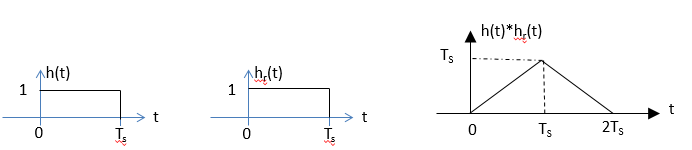
\includegraphics[width=10cm]{figure2.png}
\caption{Produit de convolution entre $h(t)$ et $h_r(t)$.}
\label{prod_conv1}
\end{figure}

\subsection{Etude théorique}

    \begin{enumerate}
        \item Calculer la densité spectrale de puissance (DSP) du signal transmis. Quelle est, en théorie, la bande nécessaire à la transmission d'un tel signal ?
        \item La chaîne de communication peut-elle vérifier le critère de Nyquist ? Justifiez votre réponse.
        \item Sans bruit, tracer le signal $z(t)$ en sortie du filtre de réception $h_r(t)$ pour la suite de bits émise suivante : $0110100$. Retrouve-t-on sur ce signal le fait que la chaine de transmission puisse respecter le critère de Nyquist ?
        \item Toujours sans bruit, tracer le diagramme de l'oeil avec une base de temps de $T_s$. Retrouve-t-on sur le diagramme de l'oeil le fait que la chaine de transmission puisse respecter le critère de Nyquist ?
        \item En supposant que l'on échantillonne aux instants optimaux (sans ISI), calculer le rapport signal sur bruit aux instants d'échantillonnage (on admettra que la puissance du bruit échantillonné et filtré est identique à celle du bruit filtré et on calculera donc cette puissance en sortie du filtre de réception).
        \item On choisira d'utiliser un détecteur à seuil. Déterminer le seuil optimal à utiliser en expliquant votre choix.
        \item En supposant que l'on échantillonne aux instants optimaux et que l'on utilise le seuil optimal de décision, donner le taux d'erreur binaire de la transmission en fonction de $T_s$ et $\sigma$, $\sigma^2$ représentant la puissance du bruit en sortie du filtre de réception $h_r(t)$.
        \item Calculer la puissance du bruit en sortie du filtre de réception $\sigma^2$ en fonction de $N_0$ et de $T_s$.
        \item Calculer l'énergie des symboles à l'entrée du récepteur, $E_s$, en fonction de $T_s$.
        \item Déduire des questions précédentes l'expression du taux d'erreur binaire (TEB) en fonction de $E_b/N_0$ pour la chaine étudiée.
    \end{enumerate}

\subsection{Implantation sous Matlab (cette chaine servira de chaine de référence pour la suite)}
    \begin{enumerate}
        \item Générer dans un premier temps le signal à transmettre en tronquant la bande occupée à une fréquence maximale égale à $\frac{4}{T_s}$. En utilisant un périodogramme estimer puis tracer la densité spectrale de puissance du signal transmis. Expliquer le résultat obtenu.
        \item Implantation de la chaine sans bruit :
            \begin{enumerate}
                \item Tracer le signal en sortie du filtre de réception. Ce tracé est-il conforme à ce que vous attendiez (voir étude théorique) ?
                \item Tracer un diagramme de l'oeil en sortie du filtre de réception afin de déterminer les instants optimaux d'échantilllonnage. Les résultats obtenus sont-ils conformes à la théorie ? Expliquez votre réponse.
                \item En utilisant les instants optimaux d'échantillonnage puis un détecteur à seuil, avec seuil optimal, vérifier que le TEB obtenu est bien nul.
            \end{enumerate}
        \item Implantation de la chaine avec bruit : rajouter le bruit et tracer le taux d'erreur binaire obtenu en fonction du rapport signal à bruit par bit à l'entrée du récepteur ($E_b/N_0$) en décibels\footnote{Attention les TEBs devront être tracés en échelle log et on fera attention à la précision des mesures réalisées (voir en annexe)}. On prendra des valeurs de $\left(E_b/N_0\right)_{dB}$ allant de $0$ à $6$ dB.
        \item Comparer le TEB simulé au TEB théorique de la chaine étudiée (tracé superposés sur une même figure). Ce tracé doit permettre de valider le bon fonctionnement de votre chaine de transmission. La fonction $Q(x)$ peut-être obtenue sou Matlab en utilisant \emph{qfunc.m}.\\
    \end{enumerate}

%%%%%%%%%%%%%%%%%%%%%%%%%%%%%%%%%%%%%%%%%%%%%%%%%%%%%%%%%%%%%%%%%%
\section{Deuxième chaine à étudier : impact du choix du filtre de réception}
%%%%%%%%%%%%%%%%%%%%%%%%%%%%%%%%%%%%%%%%%%%%%%%%%%%%%%%%%%%%%%%%%%
On considèrera un mapping binaire à moyenne nulle (symboles $a_k \in \left\{-1,1\right\}$) et les réponses impulsionnelles des filtres de mise en forme et de réception, $h(t$) et $h_r(t)$, données par la figure \ref{rep_imp_ex1_2}. Le résultat du produit de convolution entre $h(t)$ et $h_r(t)$ est donné dans la figure \ref{prod_conv}.

\begin{figure}[ht!]
\centering
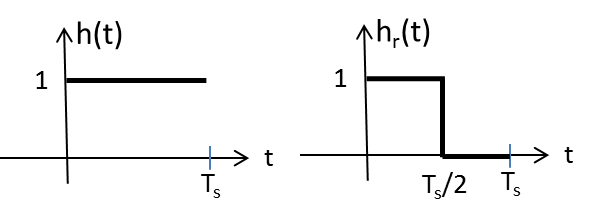
\includegraphics[width=6cm]{figure3.png}
\caption{Réponses impulsionnelles des filtres d'émission et de réception.}
 \label{rep_imp_ex1_2}
\end{figure}

\begin{figure}[ht!]
\centering
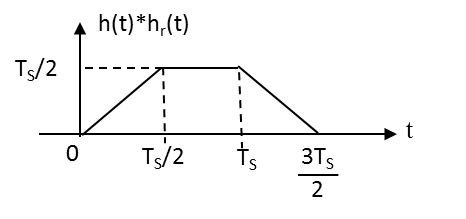
\includegraphics[width=6cm]{figure6.png}
\caption{Produit de convolution entre $h(t)$ et $h_r(t)$.}
\label{prod_conv}
\end{figure}

\subsection{Etude théorique}

    \begin{enumerate}
        \item La chaîne de communication peut-elle vérifier le critère de Nyquist ? Justifiez votre réponse.
        \item Sans bruit, tracer le signal $z(t)$ en sortie du filtre de réception $h_r(t)$ pour la suite de bits émise suivante : $0110100$. Retrouve-t-on sur ce signal le fait que la chaine de transmission puisse respecter le critère de Nyquist ? Expliquez votre réponse.
        \item Toujours sans bruit, tracer le diagramme de l'oeil avec une base de temps de $T_s$. Retrouve-t-on sur le diagramme de l'oeil le fait que la chaine de transmission puisse respecter le critère de Nyquist ? Justifiez votre réponse.
        \item En supposant que l'on échantillonne aux instants optimaux (sans ISI), calculer le rapport signal sur bruit aux instants d'échantillonnage (on admettra que la puissance du bruit échantillonné et filtré est identique à celle du bruit filtré et on calculera donc cette puissance en sortie du filtre de réception). Comparer le rapport signal sur bruit obtenu ici avec celui obtenu dans la chaine de référence. Que peut-on supposer sur la comparaison des TEBs des deux chaines de transmission ?
        \item On choisira d'utiliser un détecteur à seuil. Déterminer le seuil optimal à utiliser en expliquant votre choix.
        \item En supposant que l'on échantillonne aux instants optimaux et que l'on utilise le seuil optimal de décision, donner le taux d'erreur binaire de la transmission en fonction de $T_s$ et $\sigma$, $\sigma^2$ représentant la puissance du bruit en sortie du filtre de réception $h_r(t)$.
        \item Calculer la puissance du bruit en sortie du filtre de réception $\sigma^2$ en fonction de $N_0$ et de $T_s$.
        \item Calculer l'énergie des symboles à l'entrée du récepteur, $E_s$, en fonction de $T_s$.
        \item Déduire des questions précédentes l'expression du taux d'erreur binaire en fonction de $E_b/N_0$ pour la chaine étudiée.
    \end{enumerate}

\subsection{Implantation sous Matlab}
    \begin{enumerate}
        \item Implantation de la chaine sans bruit (le signal à transmettre sera généré en tronquant la bande occupée à une fréquence maximale égale à $\frac{4}{T_s}$)
            \begin{enumerate}
                \item Tracer le signal en sortie du filtre de réception. Ce tracé est-il conforme à ce que vous attendiez (voir étude théorique) ?
                \item Tracer un diagramme de l'oeil en sortie du filtre de réception afin de déterminer les instants optimaux d'échantilllonnage. Les résultats obtenus sont-ils conformes à la théorie ? Expliquez votre réponse.
                \item En utilisant les instants optimaux d'échantillonnage puis un détecteur à seuil, avec seuil optimal, vérifier que le TEB obtenu est bien nul.
            \end{enumerate}
        \item Implantation de la chaine avec bruit : rajouter le bruit et tracer le taux d'erreur binaire obtenu en fonction du rapport signal à bruit par bit à l'entrée du récepteur ($E_b/N_0$) en décibels. On prendra des valeurs de $\left(E_b/N_0\right)_{dB}$ allant de $0$ à $6$ dB.
        \item Comparer le TEB simulé au TEB théorique de la chaine étudiée (tracé superposés sur une même figure). Ce tracé doit permettre de valider le bon fonctionnement de votre chaine de transmission.\\
        \item Comparer le TEB obtenu par simulation pour la chaine de transmission étudiée au TEB obtenu par simulation (ou au TEB théorique) de la chaine de référence (comparaison en termes d'efficacité en puissance). La similitude ou différence obtenue devra être expliquée. La chaine éventuellement la plus efficace en puissance devra être identifiée, en expliquant pourquoi.\\
        \item Comparer l'efficacité spectrale de la chaine étudiée avec celle de la chaine de référence (en traçant, par exemple, les DSPs des signaux transmis dans les deux cas pour un même débit binaire). La similitude ou différence obtenue devra être expliquée. La chaine éventuellement la plus efficace spectralement devra être identifiée, en expliquant pourquoi.\\
    \end{enumerate}

%%%%%%%%%%%%%%%%%%%%%%%%%%%%%%%%%%%%%%%%%%%%%%%%%%%%%%%%%%%%%%%%%%
\section{Troisième chaine à étudier : impact du choix du filtre de mise en forme et d'un canal de propagation à bande limitée}
%%%%%%%%%%%%%%%%%%%%%%%%%%%%%%%%%%%%%%%%%%%%%%%%%%%%%%%%%%%%%%%%%%
On considèrera un mapping binaire à moyenne nulle (symboles $a_k \in \left\{-1,1\right\}$) et des réponses impulsionnelles des filtres de mise en forme et de réception, $h(t$) et $h_r(t)$, en racine de cosinus surélevé de même roll off $\alpha=0.5$. Le résultat du produit de convolution entre $h(t)$ et $h_r(t)$ est donc un cosinus surélevé de roll off $0.5$.

\subsection{Etude théorique}

    \begin{enumerate}
        \item La chaîne de communication peut-elle vérifier le critère de Nyquist ? Justifiez votre réponse.
        \item La chaîne de communication vérifie t-elle le critère de filtrage adapté ? Justifiez votre réponse.
        \item Donner (sans le calculer) le taux d'erreur binaire théorique de la transmission, en justifiant votre choix de formule.
        \item A quelle condition, sur le rythme symbole $R_s$, pourrait-on transmettre le signal généré par le modulateur proposé dans un canal de transmission idéal de bande $BW=1500$ Hz, tout en continuant de respecter le critère de Nyquist ?
        \item Afin d'implanter la chaine de transmission en numérique, quelle est la fréquence d'échantillonnage minimum à utiliser ? En déduire le facteur de suréchantillonnage minimal à utiliser.
    \end{enumerate}

\subsection{Implantation sous Matlab}

    \begin{enumerate}
        \item On utilisera les paramètres suivants : fréquence d'échantillonnage $F_e=12000$ Hz, rythme symbole $R_s=3000$ symboles par seconde, roll off du filtre de mise en forme et du filtre de réception $\alpha=0.5$.
        \item Implantation de la chaine sans bruit :
            \begin{enumerate}
                \item Le facteur de suréchantillonnage utilisé ici permet-il de respecter la condition d'échantillonnage de Shannon ? Justifiez votre réponse.
                \item Tracer le signal en sortie du filtre de réception. Ce tracé est-il conforme à ce que vous attendiez (voir étude théorique) ? Expliquez votre réponse.
                \item Tracer un diagramme de l'oeil en sortie du filtre de réception afin de déterminer les instants optimaux d'échantilllonnage. Les résultats obtenus sont-ils conformes à la théorie ? Justifiez votre réponse.
                \item En utilisant les instants optimaux d'échantillonnage puis un détecteur à seuil, avec seuil optimal, vérifier que le TEB obtenu est bien nul. Attention ici aux retards introduits par les filtres de la chaine de transmission qui excèdent la durée d'un symbole.
            \end{enumerate}
        \item Implantation de la chaine avec bruit : rajouter le bruit et tracer le taux d'erreur binaire (TEB) obtenu en fonction du rapport signal à bruit par bit à l'entrée du récepteur ($E_b/N_0$) en décibels. On prendra des valeurs de $\left(E_b/N_0\right)_{dB}$ allant de $0$ à $6$ dB.
        \item Comparer le TEB simulé au TEB théorique de la chaine étudiée (tracé superposés sur une même figure). Ce tracé doit permettre de valider le bon fonctionnement de votre chaine de transmission.
        \item Comparer le TEB obtenu par simulation pour la chaine de transmission étudiée au TEB obtenu par simulation (ou au TEB théorique) de la chaine de référence (comparaison en termes d'efficacité en puissance). La similitude ou différence obtenue devra être expliquée. La chaine éventuellement la plus efficace en puissance devra être identifiée, en expliquant pourquoi.
        \item Comparer l'efficacité spectrale de la chaine étudiée avec celle de la chaine de référence (en traçant les DSPs des signaux transmis dans les deux cas pour un même débit binaire). La similitude ou différence obtenue devra être expliquée. La chaine éventuellement la plus efficace spectralement devra être identifiée, en expliquant pourquoi.\\
        \item Reprendre à la chaine de transmission sans bruit et introduire un passage dans un canal de transmission
            \begin{enumerate}
                \item de bande $BW=1500$ Hz (implanté comme un filtre passe bas de fréquence de coupure $1500$ Hz : voir TPs et projet de traitement du signal).
                \item de bande $BW=3000$ Hz (implanté comme un filtre passe bas de fréquence de coupure $3000$ Hz : voir TPs et projet de traitement du signal).
            \end{enumerate}
            Dans chaque cas tracer un diagramme de l'oeil en sortie du filtre de réception et expliquer les résultats obtenus, les différences observées. Sont-ils conformes avec votre étude théorique ?
    \end{enumerate}

%%%%%%%%%%%%%%%%%%%%%%%%%%%%%%%%%%%%%%%%%%%%%%%%%%%%%%%%%%%%%%%%%%
\section{Quatrième chaine à étudier : impact du choix du mapping}
%%%%%%%%%%%%%%%%%%%%%%%%%%%%%%%%%%%%%%%%%%%%%%%%%%%%%%%%%%%%%%%%%%
On considèrera un mapping $4$-aire à moyenne nulle (symboles $a_k \in \left\{-3, -1, 1, 3\right\}$) et des réponses impulsionnelles des filtres de mise en forme et de réception, $h(t$) et $h_r(t)$, rectangulaire de durée $Ts$.

\subsection{Etude théorique}

    \begin{enumerate}
        \item Proposer un instant optimal $t_0$ pour démarrer l'échantillonnage en expliquant votre choix. On échantillonnera alors aux instants optimaux $t_0+mT_s$, $m=0, 1, 2, ...$.
        \item En supposant que l'on utilise un détecteur à seuil pour prendre les décisions, quels sont les seuils optimaux à utiliser ? Justifiez votre réponse.
        \item On suppose que l'on échantillonne aux instants optimaux et que l'on utilise un détecteur à seuil avec seuils optimaux. En utilisant le mapping suivant : $00: -3$,  $01: -1$, $11: +1$,  $10: +3$ :
                \begin{enumerate}
                    \item Calculer la probabilité de détecter (en sortie du bloc décision) le symbole $-1$ alors que l'on a émis $-3$.
                    \item Calculer la probabilité de détecter (en sortie du bloc décision) le symbole $+1$ alors que l'on a émis $-3$.
                    \item Calculer la probabilité de détecter (en sortie du bloc décision) le symbole $+3$ alors que l'on a émis $-3$.
                    \item AN : $N_0=10^{-3} V^2/Hz$, $R_b=1$ kbps.
                    %\emph{La fonction $Q(x)=\frac{1}{\sqrt{2 \pi}}\int_x^{+ \infty} e^{-\frac{u^2}{2}}du$ est donnée par la figure \ref{Qfunc} en fin d'énoncé.}
                    \item La règle de codage choisie pour le mapping vous parait-elle intéressante ? Si oui, quel est son intérêt ?
                    \item Sachant que le taux d'erreur symbole de la liaison est donné par :
                    $$
                    TES= \frac{3}{2}Q\left(\sqrt{\frac{4}{5}\frac{E_b}{N_0}}\right)
                    $$
                    Avec la règle de codage choisie pour le mapping donnez le taux d'erreur binaire (TEB) de la liaison, en expliquant votre réponse.
                \end{enumerate}
    \end{enumerate}

\subsection{Implantation sous Matlab}
\begin{enumerate}
        \item Implantation de la chaine sans bruit : on l'implantera en utilisant le mapping suivant : $00: -3$,  $01: -1$, $10: +1$,  $11: +3$ (voir en annexe). Attention le mapping est différent de celui proposé dans l'étude théorique précédente.
            \begin{enumerate}
                \item Tracer le signal en sortie du filtre d'émission, ainsi que sa densité spectrale de puissance. Ces tracés sont-ils conformes à la théorie ?
                \item Comparer l'efficacité spectrale de la chaine étudiée avec celle de la chaine de référence (en supperposant les tracés des DSPs des signaux transmis dans les deux cas pour un même débit binaire). La similitude ou différence obtenue devra être expliquée.La chaine éventuellement la plus efficace spectralement devra être identifiée, en expliquant pourquoi.
                \item Tracer un diagramme de l'oeil en sortie du filtre de réception afin de déterminer les instants optimaux d'échantilllonnage et les seuils optimaux de décision (détecteur à seuil). Les résultats obtenus sont-ils conformes à la théorie ? Expliquez votre réponse.
                \item En utilisant les instants optimaux d'échantillonnage puis un détecteur à seuil, avec seuils optimaux, vérifier que le TEB obtenu est bien nul.
            \end{enumerate}
        \item Rajouter le bruit et tracer le taux d'erreur symbole (TES) obtenu en fonction du rapport signal à bruit par bit à l'entrée du récepteur ($E_b/N_0$) en décibels. On prendra des valeurs de $\left(E_b/N_0\right)_{dB}$ allant de $0$ à $6$ dB.
        \item Comparer le TES obtenu par simulation sur la chaine implantée au TES donné pour la chaine étudiée dans l'étude théorique. La similitude ou différence obtenue devra être expliquée.
        \item Tracer le taux d'erreur binaire (TEB) obtenu en fonction du rapport signal à bruit par bit à l'entrée du récepteur ($E_b/N_0$) en décibels. On prendra des valeurs de $\left(E_b/N_0\right)_{dB}$ allant de $0$ à $6$ dB.
        \item Comparer le TEB obtenu par simulation sur la chaine implantée au TEB donné pour la chaine étudiée dans l'étude théorique. La similitude ou différence obtenue devra être expliquée. La chaine éventuellement la plus efficace en puissance devra être identifiée, en expliquant pourquoi.\\
    \end{enumerate}

\section{Conclusion}
\textcolor{blue}{A compléter}

\section{Références}
\textcolor{blue}{A compléter}

\end{document}
